%!TEX root = ../../../adrien_gomar_phd.tex

The same topology and number of grid points is used to
mesh this high-speed configuration. 
If nothing particular is said, the same numerical parameters
are kept for the study of this
high-speed configuration.
The reader is referred to 
Sec.~\ref{sec:dream_ls_numerical} for detailed information.

The same numerical approach as the low-speed configuration
is chosen for the aeroelastic computations that will
be presented in
Sec.~\ref{sec:dream_hs_ael_results}.
For practical reasons, the harmonic balance computations are run with
the same number of frequencies as the low-speed configuration,
namely five frequencies in total. This might be not sufficient
as suggested by the prediction tool shown bellow in 
Sec.~\ref{sec:dream_hs_spectral_convergence}. A partial 
convergence study is therefore conducted afterwards 
in Sec.~\ref{sub:dream_hs_convergence_ael}.
In the rear rotor,
the harmonics of the front rotor blade passing frequency
are chosen. In the front rotor, the first frequency is the
frequency associated to the vibration of the blade and the
remaining ones are the harmonics of the rear rotor blade 
passing frequency. 
The time instances are automatically chosen using the OPT
algorithm which leads to 
a condition number always lower than $1.1$, ensuring thus
the stability of the computations.

\paragraph{Influence of the spatial discretization}
\label{sub:dream_hs_spatial_discretization}

The same exercise as done in 
Sec.~\ref{sub:dream_ls_spatial_discretization} is made below
Four schemes are evaluated based 
on the convergence of the computations
and of the integrated 
results (similarity coefficients).
For the \citet{Jameson1981} scheme, the artificial viscosities
are chosen as follow: $\kappa_2 = 1.0$
and $\kappa_4 = 0.016$. We will see that the computation converges
with this low $\kappa_4$ coefficient. Therefore, only this coefficient
will be tested.

The convergence of the computations using the four spatial schemes
is reported in Figure~\ref{fig:DREAM_HS_RESIDUALS_PPT}. The convergence is good
for all the spatial schemes. In fact, more than five orders of magnitude
are lost on the residuals.
\begin{figure}[htp]
  \centering
  \includegraphics*[width=0.50\textwidth]{SPACE_SCHEME_DIFF_HS_RESIDUALS.pdf}
  \caption{High-speed isolated configuration: convergence 
  of steady computations using different spatial schemes.}
  \label{fig:DREAM_HS_RESIDUALS_PPT}
\end{figure}

The values of the similarity coefficients obtained with
all the spatial schemes is reported in 
Figure~\ref{fig:dream_hs_space_scheme_coeff}. Arbitrarily, the values are
given as a ratio over the Roe~2 values. The first-order
upwind scheme (Roe~1) give similarity coefficients that are
several percent lower than the Roe~2 value. The other schemes
give results that are less than 1\% close, therefore and for
consistence with the approach retained for the low-speed configuration
the Roe~2 scheme is chosen for the following computations.
\begin{figure}[htp]
  \centering
  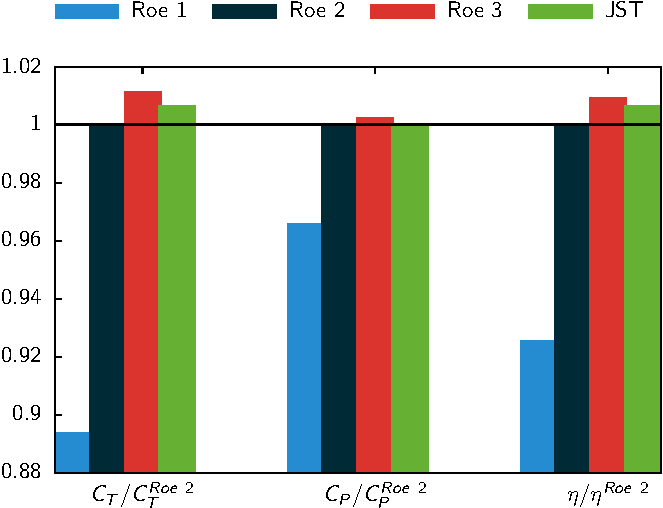
\includegraphics[width=.5\textwidth]{SPACE_SCHEME_DIFF_HS_COEFF.pdf}
  \caption{High-speed isolated configuration: convergence of 
  similarity coefficients using different spatial schemes.}
  \label{fig:dream_hs_space_scheme_coeff}
\end{figure}

